%!TEX root = ../../../_main.tex
\subsection{Residuums}
\label{sec:twisted-involutions-residuums}

\begin{defi}
	\typedlabel{defi:residuum}
	Let $w \in W$ and $I \subseteq S$ be a subset of generators. Then we define
	$$ wC_I := \{ w \ul{s_1} \ldots \ul{s_k} : k \in \nn_0, s_i \in S \} $$
	as the \defword{$I$-residuum} of $w$ or just \defword{residuum}. To emphasize the size of $I$, say $|I| = n$, we will also speak of a \defword{rank-$n$-residuum}.
\end{defi}

\begin{exam}
	Let $w \in W$. Then $wC_\emptyset = \{ w \}$ and $wC_S = \ti{\theta}$.
\end{exam}

\begin{lemm}
	\typedlabel{lemm:all-elements-of-one-residuum-yield-the-same-residuum}
	Let $w \in W$ and $I \subset S$. If $v \in wC_I$, then $vC_I = wC_I$.

	\begin{proof}
		Suppose $v \in wC_I$. Then $v = w \ul s_1 \ldots \ul s_n$ for some $s_i \in I$. Suppose $u = w \ul t_1 \ldots \ul t_m \in wC_I$ is any other element in $wC_I$ with $t_i \in I$. Then
		$$ u = w \ul t_1 \ldots \ul t_m = (v \ul s_n \ldots \ul s_1) \ul t_1 \ldots \ul t_m $$
		and so $u \in vC_I$. This yields $wC_I \subset vC_I$. Since $w \in vC_I$ we can swap $v$ and $w$ to get the other inclusion.
	\end{proof}
\end{lemm}

\begin{coro}
	Let $v, w \in W$ and $I \subset S$. Then either $vC_I \cap wC_I = \emptyset$ or $vC_I = wC_I$.

	\begin{proof}
		Immediatly follows from \ref{lemm:all-elements-of-one-residuum-yield-the-same-residuum}.
	\end{proof}
\end{coro}

\begin{prop}
	\typedlabel{prop:residuums-have-unique-wk-theta-minimal-element}
	Let $w \in \ti{\theta}$, $I \subseteq S$ be a set of generators. Then there exists a unique element $w_0 \in wC_I$ with $w_0 \preceq w_0 \ul s$ for all $s \in I$.

	\begin{proof}
		Suppose there is no such element. Then for each $w \in wC_I$ we can find a $s \in I$ with $w' = w \ul s \preceq w$ and $e' \in wC_I$. By repetition \ref{prop:deletion-property-for-twisted-expressions} says, that $e \in wC_I$, but $e$ has the property, which we assumed, that no element in $wC_I$ has. Hence there must be at least one such element. Now suppose there are two distinct elements $u,v$ with the desired property. Note that this means, that $u$ and $w$ have no reduced twisted expression ending with $\ul s \in I$. Let $v$ have a reduced twisted expression $v = \ul {s_1 \ldots s_k}$. Since $u$ and $v$ are both in $wC_I$ there must be a twisted $v$-expression for $u$
		$$ u = v \ul{ s_{k+1} \ldots s_{k+l} } = \ul{ s_1 \ldots s_{k+l} } $$
		with $s_n \in I$ for $k+1 \leq n \leq k+l$. This twisted expression cannot be reduced, since it ends with $\ul{s_{k+l}} \in I$. Then \ref{prop:deletion-property-for-twisted-expressions} yields that this twisted expression contains a reduced twisted subexpression for $u$. It cannot end with $\ul s_n$ for $k+1 \leq n \leq k+l$. Hence it is a twisted subexpression of $\ul{ s_1 \ldots s_k} = v$, too. So $u \leq v$ by \ref{theo:bruhat-subexpression-characterization}. Because of symmetry it is also $v \leq u$ and so $u = v$, contradicting to our assumption $u \neq v$.
	\end{proof}
\end{prop}

\begin{coro}
	\typedlabel{coro:residuums-have-unique-minimal-element}
	Let $w \in \ti{\theta}$, $I \subseteq S$ be a set of generators and let $\rho_{min} := \{ \rho(v) : v \in wC_I \}$ be the minimal twisted length within the residuum $wC_I$. Then there is a unique element $w_{min} \in wC_I$ with $\rho(w_{min}) = \rho_{min}$. We denote this element with $\min(w,I)$.

	\begin{proof}
		It is $\min(w,I) = w_0$ from \ref{prop:residuums-have-unique-wk-theta-minimal-element}.
	\end{proof}
\end{coro}

We proceed with some properties of rank-2-residuums. Our interest in these residuums steems from the fact, that their properties are needed later in Section \ref{sec:twisted-involutions-algorithms} to construct an effective algorithm for calculating the twisted weak ordering, i.e. calculating the Hasse diagram of $Wk(\theta)$ for arbitrary Coxeter systems $(W,S)$ and Coxeter system automorphisms $\theta$.

\begin{defi}
	Let $s,t \in S$ be two distinct generators. We define:
	$$[st]^n :=
	\begin{cases}
	(st)^{\frac{n}{2}} & n \textrm{ even}, \\
	(st)^{\frac{n-1}{2}}s & n \textrm{ odd}. 
	\end{cases}$$
\end{defi}

This definition lets us rewrite rank-2-residuums. Suppose we have a fixed start element $w \in \ti{\theta}$ and two distinct generators $s,t \in S$. Then
$$ wC_{\{s,t\}} = \{ w \} \ \cup \ \{ w \ul{[st]^n} : n \in \nn \} \ \cup \ \{ w \ul{[ts]^n} : n \in \nn \}. $$
With the following propositions and corollaries we will get a much better idea of the structure of rank-2-residuums.

\begin{lemm}
	\typedlabel{lemm:rank-2-residuums-are-convex}
	Let $w \in W$ and let $s,t \in S$ two distinct generators with $m = \ord(st)$. Without loss of generality suppose $w = \min(w, \{s,t\})$. If $m < \infty$, then $wC_{\{s,t\}}$ contains a unique maximal (regarding twisted length) element $w_{max}$ and $wC_{\{s,t\}}$ consists of two geodesics from $w$ to $w_{max}$ only intersecting in those two points. If $m = \infty$ then
	$$ wC_{\{s,t\}} = \{ w \} \ \dot \cup \ \{ w \ul{[st]^n} : n \in \nn \} \ \dot \cup \ \{ w \ul{[ts]^n} : n \in \nn \}. $$

	\begin{proof}
		\todo
	\end{proof}
\end{lemm}

\begin{prop}
	\typedlabel{prop:onesided-operations-only-at-top-or-bottom-end-of-twocycle}
	\todo
	Let $w \in S$ and $s,t \in S$ two distinct generators. If $s$ operates onesided on $w$ and $w \ul s < w$, then either $w \ul{st} < w \ul{s}$ or $w \ul{t} > w$.

	\begin{proof}
		We have $\theta(s)ws = w$ and $s \in D_R(w)$. If $t \notin D_R(w)$, then we are done. So suppose $t \in D_R(w)$. This means $w \ul s \leq w$ and $w \ul t \leq w$ and \cite[Lemma 3.9]{hultman:comb-twisted-invo} yields $w \ul {st} < w$ and $w \ul {ts} < w$. If $t \in D_R(w \ul s)$, then we are done. So suppose $t \notin D_R(w \ul s)$. Then $t \in D_R(w \ul {st})$. Together with $w \ul {st} \leq w$ \cite[Lemma 3.9(2)]{hultman:comb-twisted-invo} says $(w \ul {st}) \ul t \leq w \ul t$. Finally we get
		$$ ws = w \ul s = (w \ul {st}) \ul t \leq w \ul t = wt.$$
		Since $w \ul s$ and $w \ul t$ are of same twisted length they have to be equal and therefore $s = t$ which contradicts to our assumption of two distinct generators $s$ and $t$.
	\end{proof}
\end{prop}

\begin{coro}
	\typedlabel{coro:onesided-operations-only-at-top-or-bottom-end-of-twocycle}
	\todo
	Let $w \in S$ and $s,t \in S$ two distinct generators. If $w$ is neither the unique element in $wC_{\{s,t\}}$ of smallest twisted length nor the unique (but not neseccarily existing) element of largest twisted length, then $s$ and $t$ act twosided on $w$.

	\begin{proof}
		Follows immediatly from \ref{prop:onesided-operations-only-at-top-or-bottom-end-of-twocycle}.
	\end{proof}
\end{coro}

\begin{lemm}
	\typedlabel{lemm:max-twisted-circle-height}
	Let $w \in S$, $s,t \in S$ two distinct generators and $m = \ord(st) < \infty$. Then $|wC_{\{s,t\}}| \leq 2m$.

	\begin{proof}
		\todo
	\end{proof}
\end{lemm}

%Putting \ref{coro:rank-2-residuums-have-unique-peeks}, \ref{coro:onesided-operations-only-at-top-or-bottom-end-of-twocycle} and \ref{lemm:max-twisted-circle-height} together, the structure of rank-2-residuums is heavily constrainted.

\begin{exam}
	In Figure \ref{fig:a4_s1s3-and-a4_s2s4} we see Hasse diagram of $Wk(\id)$ on the involutions in the Coxeter group $A_4$.
	\begin{figure}[ht]
		\centering
		%!TEX root = ../../_main.tex
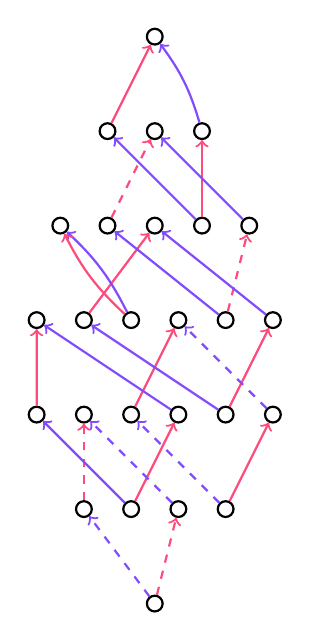
\begin{tikzpicture}[scale=0.8,bend angle=10]
\newcommand{\xspace}{1}
\newcommand{\yspace}{1}
\tikzstyle{vertex}=[draw,thick,circle,minimum size=2mm,inner sep=0pt]
\tikzstyle{edge}=[thick,->]
\tikzstyle{onesided}=[edge,dashed]
\tikzstyle{bothsided}=[edge]
\tikzstyle{unhighlighted}=[]
\tikzstyle{highlighted}=[]
\definecolor{s1color}{RGB}{130,76,253}
\definecolor{s2color}{RGB}{76,253,78}
\definecolor{s3color}{RGB}{253,76,124}
\definecolor{s4color}{RGB}{76,176,253}
\tikzstyle{s1}=[s1color]
\tikzstyle{s2}=[s2color]
\tikzstyle{s3}=[s3color]
\tikzstyle{s4}=[s4color]
\node[vertex,unhighlighted] (0) at (\xspace*0,\yspace*0) {};
\node[vertex,unhighlighted] (1) at (\xspace*-1.125,\yspace*1.5) {};
\node[vertex,unhighlighted] (2) at (\xspace*-0.375,\yspace*1.5) {};
\node[vertex,unhighlighted] (3) at (\xspace*0.375,\yspace*1.5) {};
\node[vertex,unhighlighted] (4) at (\xspace*1.125,\yspace*1.5) {};
\node[vertex,unhighlighted] (5) at (\xspace*-1.875,\yspace*3) {};
\node[vertex,unhighlighted] (6) at (\xspace*-1.125,\yspace*3) {};
\node[vertex,unhighlighted] (7) at (\xspace*-0.375,\yspace*3) {};
\node[vertex,unhighlighted] (8) at (\xspace*0.375,\yspace*3) {};
\node[vertex,unhighlighted] (9) at (\xspace*1.125,\yspace*3) {};
\node[vertex,unhighlighted] (10) at (\xspace*1.875,\yspace*3) {};
\node[vertex,unhighlighted] (11) at (\xspace*-1.875,\yspace*4.5) {};
\node[vertex,unhighlighted] (12) at (\xspace*-1.125,\yspace*4.5) {};
\node[vertex,unhighlighted] (13) at (\xspace*-0.375,\yspace*4.5) {};
\node[vertex,unhighlighted] (14) at (\xspace*0.375,\yspace*4.5) {};
\node[vertex,unhighlighted] (15) at (\xspace*1.125,\yspace*4.5) {};
\node[vertex,unhighlighted] (16) at (\xspace*1.875,\yspace*4.5) {};
\node[vertex,unhighlighted] (17) at (\xspace*-1.5,\yspace*6) {};
\node[vertex,unhighlighted] (18) at (\xspace*-0.75,\yspace*6) {};
\node[vertex,unhighlighted] (19) at (\xspace*0,\yspace*6) {};
\node[vertex,unhighlighted] (20) at (\xspace*0.75,\yspace*6) {};
\node[vertex,unhighlighted] (21) at (\xspace*1.5,\yspace*6) {};
\node[vertex,unhighlighted] (22) at (\xspace*-0.75,\yspace*7.5) {};
\node[vertex,unhighlighted] (23) at (\xspace*0,\yspace*7.5) {};
\node[vertex,unhighlighted] (24) at (\xspace*0.75,\yspace*7.5) {};
\node[vertex,unhighlighted] (25) at (\xspace*0,\yspace*9) {};
\draw[s1,onesided,unhighlighted] (0) edge (1);
\draw[s3,onesided,unhighlighted] (0) edge (3);
\draw[s3,onesided,unhighlighted] (1) edge (6);
\draw[s1,bothsided,unhighlighted] (2) edge (5);
\draw[s3,bothsided,unhighlighted] (2) edge (8);
\draw[s1,onesided,unhighlighted] (3) edge (6);
\draw[s1,onesided,unhighlighted] (4) edge (7);
\draw[s3,bothsided,unhighlighted] (4) edge (10);
\draw[s3,bothsided,unhighlighted] (5) edge (11);
\draw[s3,bothsided,unhighlighted] (7) edge (14);
\draw[s1,bothsided,unhighlighted] (8) edge (11);
\draw[s1,bothsided,unhighlighted] (9) edge (12);
\draw[s3,bothsided,unhighlighted] (9) edge (16);
\draw[s1,onesided,unhighlighted] (10) edge (14);
\draw[s3,bothsided,unhighlighted] (12) edge (19);
\draw[s1,bothsided,unhighlighted,bend right] (13) edge (17);
\draw[s3,bothsided,unhighlighted,bend left] (13) edge (17);
\draw[s1,bothsided,unhighlighted] (15) edge (18);
\draw[s3,onesided,unhighlighted] (15) edge (21);
\draw[s1,bothsided,unhighlighted] (16) edge (19);
\draw[s3,onesided,unhighlighted] (18) edge (23);
\draw[s1,bothsided,unhighlighted] (20) edge (22);
\draw[s3,bothsided,unhighlighted] (20) edge (24);
\draw[s1,bothsided,unhighlighted] (21) edge (23);
\draw[s3,bothsided,unhighlighted] (22) edge (25);
\draw[s1,bothsided,unhighlighted,bend right] (24) edge (25);
\end{tikzpicture}
		\quad \quad \quad
		\input{resources/tikz/a4_s2s4}
		\caption{Hasse diagrams of $Wk(\id), W = A_4$ with only $s_1,s_3$ edges on the left and only $s_2,s_4$ edges on the right side}
		\label{fig:a4_s1s3-and-a4_s2s4}
	\end{figure}
\end{exam}